\documentclass{article}
\usepackage{listings}
\usepackage[utf8]{inputenc}
\usepackage[T1]{fontenc}
\usepackage{geometry}
\usepackage{graphicx}
\usepackage{url}


\geometry{a4paper}

% \addtolength{\oddsidemargin}{-.875in} %
% \addtolength{\evensidemargin}{-.875in} %
% \addtolength{\textwidth}{1.55in} %
\addtolength{\topmargin}{-.875in}
\addtolength{\textheight}{2.25in}

\begin{document}

\begin{titlepage}
   \begin{center}
       \vspace*{1cm}
 
       \textbf{Trabajo Práctico Nro. 21}
 
       \vspace{0.5cm}
        Interpretación de BPFlotante IEEE 754
 
       \vspace{1.5cm}
 
       \textbf{Juan Carlos Junior Soria Flores\\103068}
 
       \vfill
 
       Organización del Computador 75.03
  
   \end{center}
\end{titlepage}

\newpage
\tableofcontents

\newpage
\section{Enunciado}
\subsection{Interpretacion de BPFlotante IEEE 754}
Se pide desarrollar un programa en assembler Intel 80x86 que lea de teclado e imprima lo siguiente:
\begin{enumerate}
\item Configuraciones binaria o hexadecimal de números almacenados en formato IEEE 754 de precisión simple $\rightarrow$ Notación científica normalizada en base 2(Ej. -1,110101 x 10$^{101}$).
\item Notaciones científicas normalizadas en base 2 $\rightarrow$ Configuraciones binaria o hexadecimal de números almacenados en formato IEEE 754 de precisión simple.
\end{enumerate}

\newpage
\section{Flujo programa}
\begin{center}
  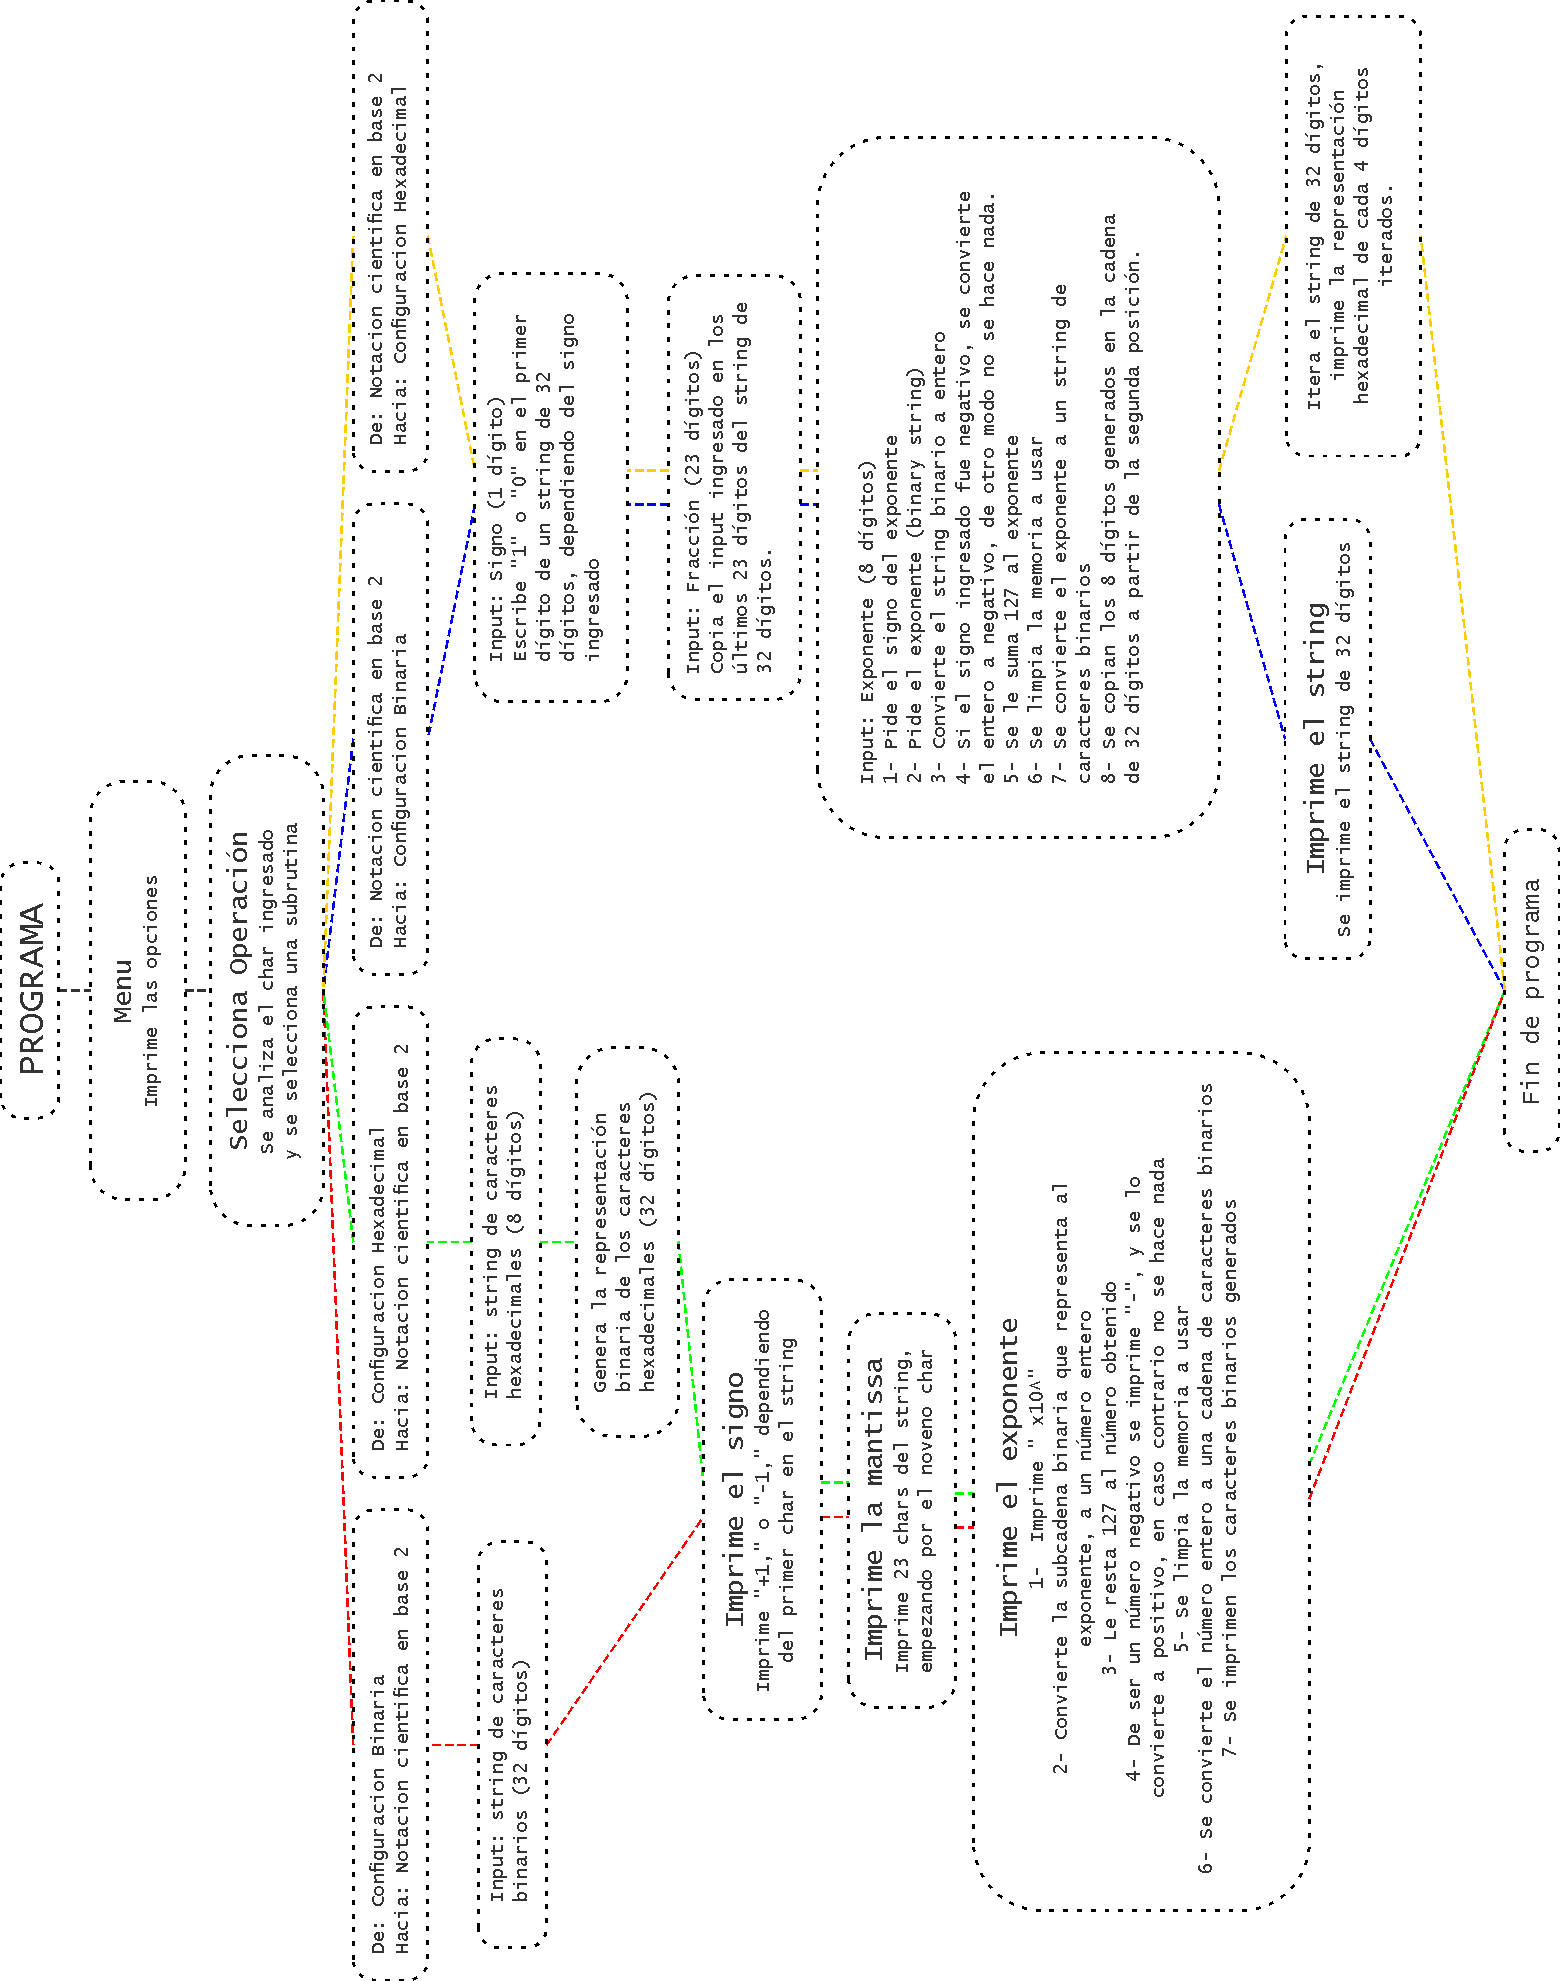
\includegraphics[scale=0.4]{diagrama.png}
\end{center}

\newpage
\section{Código}
	\subsection{macros.asm}
	\begin{verbatim}
%ifndef MACROS_ASM
%define MACROS_ASM

extern _printf
extern _gets

;Imprime un string usando un formato
%macro prints2 2  ;string , formato
        push        %1
        push        %2
        call        _printf
        add         esp,8
%endmacro

;Imprime un string que termina en cero
%macro prints 1    ;string
        push        %1
        call        _printf
        add         esp,4
%endmacro

;Pide al usuario una cantidad "len" de caracteres y la almacena en dest.
%macro getstr 3     ;temp_dest, dest, len
        jmp         %%getstrR
%%getstrERR:
        prints      me_err_len
%%getstrR:
        flush       %1,%3+1
        push        %1
        call        _gets
        add         esp,4
        cmp         byte[%1+%3],byte 0
        jne         %%getstrERR
        memcopy     %1, %2, %3
%endmacro

;Escanea una longitud predefinida de caracteres,
;de encontrarse algun di­gito invalido, coloca el valor -1 en edi.
%macro bintest 2   ;input, longitud
        mov         esi, %2
        mov         edi, -1
%%bintestR:
        inc         edi
        cmp         edi,esi
        je          %%bintestE
        mov         bl, byte [ %1 + edi]
        cmp         bl, 0x31
        je          %%bintestR
        cmp         bl, 0x30
        je          %%bintestR
        mov         edi, -1
%%bintestE:
%endmacro

;Escanea una longitud predefinida de caracteres,
;de encontrarse algun di­gito invalido, coloca el valor -1 en edi.
%macro hextest 2   ;src, len
        mov         edx,-1
        mov         edi,0
        mov         esi,0
%%hextestR:
        mov         bl, byte [%1+esi] ;muevo el char  a  BL
        sub         bl, 48  ;  le resto  48
        mov         cl, bl ; lo copio en  CL
        sub         cl, 7;  le quito 7 a  CL
        cmp         bl, 10 ; compaaro si  BL es mayor o iguaal que  10
        cmovge      ebx,ecx;  muevvo CLL a  BL
        cmp         bl, 16; comparo si  BL es mayor o iguaal que  16
        cmovge      edi,edx
        cmp         edi,-1
        je          %%hextestE
        mov         byte [%1+esi], bl
        inc         esi
        cmp         esi,%2
        je          %%hextestE
        jmp         %%hextestR
%%hextestE:
%endmacro

;Analiza si lo ingresado es + o -, de otro modo, se vuelve a solicitar input
%macro getsign 7    ;msg_beg, temp_dest, dest, len, end_dest, sign+, sign-
        jmp         %%getsign
%%getsignR:
        prints      me_err_sign
%%getsign:
        prints      %1
        getstr      %2,%3,%4
        cmp         byte[%3],0x2B
        jne         %%getsignA
        mov         byte[%5],%6
        jmp         %%getsignE
%%getsignA:
        cmp         byte[%3],0x2D
        jne         %%getsignR
        mov         byte[%5],%7
%%getsignE:
%endmacro

;Combinacion de los macros getstr y bintest fundamentalmente
%macro getbinstr 4  ;me_cfg, temp_dest, dest, len
        jmp         %%getbinstr
%%getbinstrR:
        prints      me_err_bin
%%getbinstr:
        prints      %1
        getstr      %2, %3, %4
        bintest     %3, %4
        cmp         edi, -1
        je          %%getbinstrR
%endmacro

;Combinacion de los macros getstr y hextest fundamentalmente
%macro gethexstr 4
        jmp         %%gethexstr
%%gethexstrR:
        prints      me_err_hex
%%gethexstr:
        prints      %1
        getstr      %2, %3, %4
        hextest     %3, %4
        cmp         edi, -1
        je          %%gethexstrR
%endmacro

;Testea si dos strings son iguales
%macro testspc 4 ; str, str, msg, len
        mov     esi, 0
        jmp     %%inc_esie
%%inc_esi:
        add     esi,4
        cmp     esi, %4
        je      %%pass
%%inc_esie:
        mov     ecx,dword[%1+esi]
        mov     edx,dword[%2+esi]
        cmp     ecx,edx
        je      %%inc_esi
        mov     esi,-1
        jmp     %%testzeroE
%%pass:
        mov     esi, 1
%%testzeroE:
        cmp     esi,1
        jne     %%testzeroEE
        prints  %3
%%testzeroEE:
%endmacro

;Copia una cantidad n de bytes de src en dest
%macro memcopy 3    ;src, dest, n
        mov         esi,%1
        mov         edi,%2
        mov         ecx,%3
        rep         movsb
%endmacro

;Setea una cantidad (con 0x30) n de bytes desde src
%macro flush 2      ; src, n
        mov         esi,0
%%flushR:
        mov         byte[%1+esi],0x30
        inc         esi
        cmp         esi, %2
        jne         %%flushR
%endmacro

;Convierte caracteres hexadecimales a binarios
%macro HexToBin 3   ;src, dest, src_len
        push        ebp
        mov         ebp,esp
        sub         esp, 4
        mov         edi,0
        mov         esi,0
%%nextchar:
        mov         bl, byte [%1+esi]
        mov         dword [ebp-4], 0
%%writeR:
        mov         dl, bl
        shr         dl, 3
        and         dl, 1
        mov         byte[%2+edi],byte 0x30
        cmp         dl, 1
        jne         %%writeE
        mov         byte[%2+edi],byte 0x31
%%writeE:
        shl         bl, 1
        inc         dword [ebp-4]
        inc         edi
        cmp         dword [ebp-4], 4   ;Se necesitan 4 cifras binarias
        jl          %%writeR
        inc         esi                ;Se pasa al siguiente char
        cmp         esi,%3             ;String len
        je          %%hextobinE
        jmp         %%nextchar
%%hextobinE:
        add         esp,4
        pop         ebp
%endmacro

;Imprime un caracter hexadecimal cada 4 caracteres binarios
%macro BinToHex 3   ;src, src_len, format
        mov         esi,0
%%add8:
        mov         edi,0
        mov         al, byte[%1+esi]
        inc         esi
        cmp         al, 0x31
        jne         %%add4
        add         edi,8
%%add4:
        mov         al, byte[%1+esi]
        inc         esi
        cmp         al,0x31
        jne         %%add2
        add         edi,4
%%add2:
        mov         al, byte[%1+esi]
        inc         esi
        cmp         al,0x31
        jne         %%add1
        add         edi,2
%%add1:
        mov         al, byte[%1+esi]
        inc         esi
        cmp         al,0x31
        jne         %%add0
        add         edi,1
%%add0:
        prints2     edi,%3
        cmp         esi,%2
        jne         %%add8
%endmacro

;Obtiene un numero entero decimal a partir de un string
;de caracteres binarios de longitud len y lo almacena en int
%macro BinToDec 3   ;int, string, len
        mov         esi, 0             ;iter
        mov         dword[%1], 0       ;valor dword[exp_int]
        mov         edx, 0             ;resto
        mov         eax, 128           ;dividiendo
        mov         ecx, 2             ;divisor
%%bintodecR:
        cmp         byte[%2+esi], 0x31
        jne         %%bintodecE
        add         dword[%1],eax
%%bintodecE:
        inc         esi
        div         ecx
        cmp         esi,%3
        jne         %%bintodecR
%endmacro

; Genera la representacion binaria en mem_8 del numero en exp_int
; haciendo divisiones sucesivas
%macro DecToBin 3   ;exp_int, 8, mem_8
        mov         eax, dword[%1]     ;dividiendo
        mov         esi,%2 -1
        mov         ecx, 2             ;divisor
%%dectobinR:
        mov         edx, 0
        div         ecx                ;eax contendra el cociente
        cmp         edx,0              ;edx contendra el resto
        jne         %%write1
        mov         byte[%3+esi],0x30
        jmp         %%write1E
%%write1:
        mov         byte[%3+esi],0x31

%%write1E:
        sub         esi, 1
        cmp         eax, 2
        jge         %%dectobinR
        mov         byte[%3+esi],0x31
%endmacro

%endif

	\end{verbatim}
	
	\subsection{data.asm}
	\begin{verbatim}
%ifndef DATA_ASM
%define DATA_ASM

        section .data

        me_title    db 10,10,"75.03 / 95.57 Organizacion del Computador",10,
                    db "Trabajo Practico Nro. 21 || ",
                    db "Interpretacion de BPFlotante IEEE 754",10,0
        me_menu     db 10,"1 - Configuracion Binaria -> Notacion cientifica en base 2",10,
                    db "2 - Configuracion Hexadecimal -> Notacion cientifica en base 2",10,
                    db "3 - Notacion cientifica en base 2 -> Configuracion Binaria",10,
                    db "4 - Notacion cientifica en base 2 -> Configuracion Hexadecimal",10,
                    db 10,"Ingrese el numero de operacion (1 digito)",10,0

        me_bin_cfg  db "Ingrese la configuracion binaria (32 digitos): ",10,0
        me_hex_cfg  db "Ingrese la configuracion hexadecimal (8 digitos): ",10,0

        me_bin_end1 db 10,"La configuracion binaria contiene el numero: ",10,0
        me_bin_end2 db 10,"La configuracion hexadecimal contiene el numero: ",10,0
        me_sci_end1 db 10,"La configuracion binaria es: ",10,0
        me_sci_end2 db 10,"La configuracion hexadecimal es: ",10,0

        me_sci_sign db "Ingrese el signo del numero (+/-): ",10,0
        me_sci_frac db "Ingrese la fraccion (23 di­gitos): ",10,0
        me_sci_exps db "Ingrese el signo del exponente (+/-): ",10,0
        me_sci_exp  db "Ingrese el exponente (8 di­gitos): ",10,0

        me_err_sign db "Solo es valido ingresar '+' o '-'",10,0
        me_err_op   db "Operacion invalida",10,0
        me_err_len  db "Cantidad incorrecta de caracteres",10,0
        me_err_bin  db "Solo es valido ingresar caracteres binarios",10,0
        me_err_hex  db "Solo es valido ingresar numeros y letras mayusculas",10,0

        print_inth  db "%X",0
        print_1     db "%.1s",0
        print_8     db "%.8s",0
        print_23    db "%.23s",0
        print_32    db "%.32s",0

        one_pos     db "+1,",0
        one_neg     db "-1,",0
        ten_power   db " x10^",0
        plus_symb   db "+",0
        neg_symb    db "-",0
        new_line    db 10,0

        pzerob  db "00000000000000000000000000000000",10,0
        nzerob  db "10000000000000000000000000000000",10,0
        pinfb   db "01111111100000000000000000000000",10,0
        ninfb   db "11111111100000000000000000000000",10,0
        qnanb   db "011111111",10,0
        snanb   db "111111111",10,0
        pzero   db "+0",10,0
        nzero   db "-0",10,0
        pinf    db "Infinito positivo",10,0
        ninf    db "Infinito negativo",10,0
        qnan    db "QNaN",10,0
        snan    db "SNaN",10,0

%endif

	\end{verbatim}
	
	\subsection{bss.asm}
	\begin{verbatim}
%ifndef BSS_ASM
%define BSS_ASM

        section .bss

        exp         resd 1
        mem_1       resb 1
        mem_8       resb 9
        mem_23      resb 23
        mem_32      resb 32
        string      resb 128
%endif

	\end{verbatim}


	\subsection{main.asm}
	\begin{verbatim}
%include "data.asm"
%include "macros.asm"
%include "bss.asm"

global _main
extern _ExitProcess@4

        section .text
_main:
        prints      me_title
        prints      me_menu
        call        askop
        
end:
        call        _ExitProcess@4
;_______________________________________________________________________
askopR:
        prints      me_err_op
askop:
        getstr      string, mem_1, 1
        mov         al,[mem_1]
        cmp         al,0x31
        je          op_1
        cmp         al,0x32
        je          op_2
        cmp         al,0x33
        je          op_3
        cmp         al,0x34
        je          op_4
        jmp         askopR
askopE:
        ret
;_______________________________________________________________________
op_1:
        getbinstr   me_bin_cfg, string, mem_32, 32
        prints      me_bin_end1
        call        specialtest
        cmp         esi,1
        je          op_1E
        call        printsign
        prints2     mem_32 +9, print_23
        call        printexp
op_1E:
        jmp         askopE

op_2:
        gethexstr   me_hex_cfg, string, mem_8, 8
        prints      me_bin_end2
        HexToBin    mem_8, mem_32, 8
        call        specialtest
        cmp         esi, 1
        je          op_2E
        call        printsign
        prints2     mem_32 +9, print_23
        call        printexp
op_2E:
        jmp         askopE

op_3:
        getsign     me_sci_sign, string, mem_1, 1, mem_32, 0x30, 0x31
        getbinstr   me_sci_frac, string, mem_32+9, 23
        call        getexp
        prints      me_sci_end1
        prints2     mem_32, print_32
        prints      new_line
        jmp         askopE

op_4:
        getsign     me_sci_sign, string, mem_1, 1, mem_32, 0x30, 0x31
        getbinstr   me_sci_frac, string, mem_32+9, 23
        call        getexp
        prints      me_sci_end2
        BinToHex    mem_32, 32, print_inth
        prints      new_line
        jmp         askopE
;_______________________________________________________________________
;  Imprime (+1/-1) dependiendo
;  de lo almacenado en mem_32
printsign:
        mov         eax,one_neg
        mov         edx,one_pos
        cmp         byte[mem_32],0x30
        cmove       eax,edx
        prints      eax
        ret
;_______________________________________________________________________
;   Convierte el exponente binario a decimal
;   Le resta 127 para obtener el valor original
;   Imprime el signo en caso de ser nagativo
;   y lo convierte en positivo.
;   Convierte el valor decimal, en binario y lo muestra
printexp:
        prints      ten_power
        BinToDec    exp, mem_32+1, 8
        sub         dword[exp],127
        call        showexpsign
        flush       mem_8, 8
        DecToBin    exp, 8, mem_8
        call        printexpA
        prints      new_line
        ret
;______________________________________________________________________
;   Imprime el signo del exponente y convierte el exponente a positivo
showexpsign:
        cmp         dword[exp],0
        jge         showexpsignE
        prints      neg_symb
        neg         dword[exp]
showexpsignE:
        ret
;_______________________________________________________________________
;   Imprime el exponente filtrando los ceros del comienzo
printexpA:
       mov byte[mem_8+8],0
       mov esi,0
       jmp inc_esie
inc_esi:
       inc esi
inc_esie:
       cmp byte[mem_8+esi],0x30
       je  inc_esi
       mov edx,mem_8
       add edx,esi
       prints edx
       ret
;_______________________________________________________________________
;   Rutina para pedir informacion del exponente, convertirlo a decimal,
;   convertir el decimal en negativo (si el signo ingresado para
;   el exponente es negativo), sumarle 127 (porque sera almacenado
;   en exceso 127), convertir el decimal en binario y almacenar
;   esta ultima configuracion en mem_32+1
getexp:
        getsign     me_sci_exps, string, mem_1, 1, mem_1, 0x2B, 0x2D
        getbinstr   me_sci_exp, string, mem_8, 8
        memcopy     mem_8, mem_32+1,8
        BinToDec    exp, mem_32+1, 8
        call        expchecksign
        add         dword[exp],127
        flush       mem_8, 8
        DecToBin    exp, 8, mem_8
        memcopy     mem_8, mem_32+1,8
        ret
;_______________________________________________________________________
;   Si el signo ingresado para el exponente es negativo,
;   se convierte el exponente decimal a negativo
expchecksign:
        cmp         byte[mem_1],0x2B
        je          expchecksignE
        neg         dword[exp]
expchecksignE:
        ret
;______________________________________________________________________
;   Testea los valores especiales de IEEE 754
specialtest:
        testspc   mem_32, pzerob, pzero, 32
        cmp       esi,1
        je        specialtestE
        testspc   mem_32, nzerob, nzero, 32
        cmp       esi,1
        je        specialtestE
        testspc   mem_32, pinfb, pinf, 32
        cmp       esi,1
        je        specialtestE
        testspc   mem_32, ninfb, ninf, 32
        cmp       esi,1
        je        specialtestE
        testspc   mem_32, qnanb, qnan, 8
        cmp       esi,1
        je        specialtestE
        testspc   mem_32, snanb, snan, 8
specialtestE:
        ret

	\end{verbatim}

\newpage
\section{Compilación}
El programa fue desarrollado bajo $Windows \; 10$, no obstante, se provee el código para que pueda ser ensamblado bajo $Linux$. Se usó $NASM$ como ensamblador, $SASM$ como debugger y $Atom$ como editor de texto.
\subsection{Ensamblado}
Parametros NASM:
\begin{verbatim}
nasm main.asm -f win32 -o main.o
\end{verbatim}
\subsection{Linkedición}
Parametros GCC:
\begin{verbatim}
gcc main.o -m32 -o tp21
\end{verbatim}
\subsection{Ejecución}
Comando:
\begin{verbatim}
./tp21
\end{verbatim}


\newpage
\section{Pruebas realizadas}
Para verificar el correcto funcionamiento se realizaron varias pruebas, ya sea para validar lo que el usuario ingresa, y verificar los resultados.

\subsection{Configuración Binaria $\rightarrow$ Notación científica en base 2}
\begin{lstlisting}[mathescape]
a) $01111000011111111111111111111110  \rightarrow  1.11111111111111111111110 \cdot 10^{1110001}$
b) $01010101010101010101010101010101 \rightarrow 1.10101010101010101010101 \cdot 10^{101011} $
c) $10000111100000000000000000000000  \rightarrow  -1.00000000000000000000000 \cdot 10^{-1110000}$
d) $00000000000000000000000000000000  \rightarrow +0.0$
e) $10000000000000000000000000000000  \rightarrow  -0.0$
f) $01111111100000000000000000000000   \rightarrow  Infinito\; positivo$
f) $11111111100000000000000000000000   \rightarrow  Infinito\; negativo$
g) $01111111100000000000000000000001  \rightarrow QNan$
h) $11111111100000000000000000000001  \rightarrow SNan$
\end{lstlisting}

\subsection{Configuración Hexadecimal $\rightarrow$ Notación científica en base 2}
\begin{lstlisting}[mathescape]
a) $787FFFFE  \rightarrow  1.11111111111111111111110 \cdot 10^{1110001}$
b) $55555555  \rightarrow 1.10101010101010101010101 \cdot 10^{101011} $
c) $87800000  \rightarrow  -1.00000000000000000000000 \cdot 10^{-1110000}$
d) $00000000  \rightarrow +0.0$
e) $80000000  \rightarrow  -0.0$
f) $7F800000   \rightarrow  Infinito\; positivo$
f) $FF800000   \rightarrow  Infinito\; negativo$
g) $7F800001  \rightarrow QNan$
h) $FF800001  \rightarrow SNan$
\end{lstlisting}

\subsection{Notación científica en base 2 $\rightarrow$ Configuración Binaria}
\begin{lstlisting}[mathescape]
a) $1.11111111111111111111110 \cdot 10^{1110001} \rightarrow 01111000011111111111111111111110   $
b) $1.10101010101010101010101 \cdot 10^{101011} \rightarrow 01010101010101010101010101010101$
c) $-1.00000000000000000000000 \cdot 10^{-1110000} \rightarrow 10000111100000000000000000000000$
\end{lstlisting}

\subsection{Notación científica en base 2 $\rightarrow$ Configuración Hexadecimal}
\begin{lstlisting}[mathescape]
a) $1.11111111111111111111110 \cdot 10^{1110001} \rightarrow 787FFFFE   $
b) $1.10101010101010101010101 \cdot 10^{101011} \rightarrow 55555555$
c) $-1.00000000000000000000000 \cdot 10^{-1110000} \rightarrow 87800000$
\end{lstlisting}

\newpage
\section{Comentarios}
\subsection{Archivos adicionales bajo Linux}
Para poder ensamblar usando instrucciones de 32 bits, bajo Linux, se necesitan instalar archivos adicionales. Bajo Ubuntu 18.04 se usó el siguiente comando:
\begin{verbatim}
sudo apt install gcc-multilib
\end{verbatim}
\subsection{Manejo de entrada}
El programa es capaz de manejar entrada errónea del usuario.
\subsection{Beneficios Linux}
Algunos beneficios encontrados al usar Linux como plataforma de desarrollo fueron:
\begin{enumerate}
\item Mayor facilidad al encontrar errores.
\item Linux mostró ser más susceptible a errores, por lo cual, tales errores fueron corregidos más pronto.
\item Linux permite imprimir carácteres con tildes.
\item El uso nativo de Makefile.
\end{enumerate}
\subsection{Código en la nube}
\begin{verbatim}
http://bit.ly/2WP6rqU
\end{verbatim}
\end{document}